\chapter{METODOLOGIA E AVALIAÇÃO}

As discussões sobre os processos de formação no Ensino Superior têm destacado a relação entre conhecimento e ensino no contexto de uma transição paradigmática das Ciências que, dentre outros aspectos, se caracteriza pela emergência de sistemas de conhecimento abertos e não dicotômicos (SANTOS, 1988). Segundo Cunha (2005, p. 13), o “paradigma emergente” nas Ciências situa os professores do magistério superior diante de novos desafios, a saber:

\begin{enumerate}[label=(\alph*)]
    \item Enfoque no conhecimento a partir da historicidade de sua produção e de sua provisoriedade e relatividade;
    \item Estímulo à análise, à capacidade de composição de dados, informações, argumentos e ideias;
    \item Valorização da curiosidade, do questionamento e da incerteza;
    \item Percepção do conhecimento como interdisciplinar, estabelecendo relações e atribuição de significados em função dos objetivos sociais e acadêmicos;
    \item Valorização da pesquisa como um instrumento do ensino e a extensão como ponto de partida e chegada da apreensão da realidade;
    \item Valorização das habilidades sócio-intelectuais tanto quanto os conteúdos.
\end{enumerate}

Neste contexto, a docência assume um novo papel deslocando-se do modelo onde figurava como fonte da informação para uma posição de mediação entre o aluno e o seu objeto de conhecimento. O destaque dado à importância da autonomia do estudante em seu processo de desenvolvimento intelectual, social e afetivo põe em relevo o protagonismo do processo de ensino e aprendizagem na consecução dos objetivos do curso (seção 4), considerando o perfil do egresso (seção 5) e as respectivas competências e habilidades esperadas de um Bacharel em Ciência da Computação. Diante disso, este projeto orienta-se por determinadas concepções teórico-metodológicas, tendo em vista possibilitar a execução do escopo almejado.

\section{Concepção de ensino e aprendizagem}

O ensino e a aprendizagem são compreendidos como elementos constituintes de um mesmo processo de construção do conhecimento em que o aluno e seu objeto de estudo estão em contínua relação mediados pela ação do professor (ANASTASIOU; ALVES, 2015). Isso significa que o ensino não corresponde a uma transmissão de informações, mas assume um caráter dialógico, problematizador e contextualizador do próprio objeto de conhecimento (FREIRE, 2005b). O professor age de modo a estimular a aprendizagem, valorizando os conhecimentos prévios dos alunos, proporcionando-lhes experiências de pesquisa, interação social e expressão de saberes, práticas, atitudes e valores, ao mesmo tempo em que avalia permanentemente o seu desenvolvimento.

Nessa concepção, os conteúdos da aprendizagem não se apresentam isolados de sua dimensão epistemológica, social ou política. Além disso, tais conteúdos são abrangentes, incluindo fatos, conceitos, procedimentos e atitudes (ZABALA, 1998). O professor deve, então, fomentar, junto aos seus alunos, momentos que estimulem a apreensão da complexidade inerente ao objeto de estudo por meio da problematização. O processo de ensino-aprendizagem numa perspectiva ativa, e não mecânica ou “bancária” (FREIRE, 2005a), coloca o aluno como protagonista de seu desenvolvimento intelectual, social e afetivo ao mobilizar seu potencial para responder aos desafios postos pelos novos saberes (BERBEL, 2011). Tal postura favorece uma “aprendizagem significativa” em que os novos conhecimentos interagem de maneira substantiva, ou seja, não literal, com os conhecimentos já construídos pelo aluno. Neste sentido, trata-se de uma aprendizagem não arbitrária, pois se apoia nos conhecimentos prévios dos alunos tornando-os mais ricos ou dotados de novos significados, de modo a estimular a criatividade e autonomia (MOREIRA, 2010).

Compreendido desta forma, o processo de ensino-aprendizagem possibilita considerar a tríade professor-conhecimento-aluno a partir de novas perspectivas. Por exemplo, as concepções de espaço e tempo do ensinar e do aprender distanciam-se da tradicional clivagem entre ensino presencial e virtual em prol de uma concepção híbrida possibilitando, assim, o uso planejado das mais variadas tecnologias digitais aliadas a uma interação entre o aluno e o grupo-classe.

\section{As Tecnologias da Informação e Comunicação – TICs aplicadas ao ensino e a aprendizagem}

O ensino híbrido representa uma quebra de paradigmas em direção a uma proposta de inovação mais alinhada com os avanços tecnológicos de uma sociedade pós-moderna. Pensar o ensino híbrido, portanto, significa organizar estratégias metodológicas utilizando atividades presenciais e a distância em plataformas on-line, empregando TICs, e off-line, nos momentos de interação com colegas e/ou com o professor/tutor. Segundo Christensen, Horn e Staker (2013), no ensino híbrido, o aluno aprende:

\begin{citacao}
    “Pelo menos em parte por meio do ensino online, com algum elemento de controle do estudante sobre o tempo, local, caminho e/ou ritmo de estudo e, pelo menos em parte, em uma localidade física supervisionada, fora de sua residência. As modalidades ao longo do caminho de aprendizado de cada estudante em um curso ou matéria são conectadas para oferecer uma experiência de educação integrada”.
\end{citacao}

Nessa perspectiva, seja presencialmente ou à distância, o estudante compartilha de espaços interativos e integrativos de aprendizagem. São exemplos de uma abordagem híbrida do ensino (BACICH; NETO; TREVISANI, 2015):

\noindent \textbf{Sala de aula invertida}: o aluno estuda a teoria em casa utilizando-se de plataforma on-line; o tempo e o espaço da sala de aula são utilizados para discussões e realização de atividades. Os assuntos são disponibilizados previamente pelo professor no Ambiente Virtual de Aprendizagem – AVA. No momento da aula, os alunos compartilham com o professor suas observações a respeito do material estudado previamente e, seguindo, um plano de trabalho, desenvolvem atividades relacionadas com a teoria, com uso das mais variadas estratégias: rotação por estações, laboratório rotacional, seminários, estudos de caso, etc.

\noindent \textbf{Rotação por estações}: os alunos são divididos em grupos (estações), cada qual realizando uma determinada tarefa, tendo em vista os objetivos definidos no plano de aula. Um dos grupos estará, necessariamente, desenvolvendo alguma atividade de forma on-line. Após transcorrer um determinado período, os alunos trocam de grupo, de modo a trabalhar em uma tarefa diferente da sua. Este revezamento continua até que todos os estudantes tenham passado por todos os grupos. 

Ainda que as atividades realizadas em cada grupo sejam independentes, no final, elas funcionam de forma integrada, possibilitando, assim, uma compreensão de conjunto do objeto estudado.

\noindent \textbf{Laboratório rotacional}: é semelhante ao modelo da rotação por estações, mas, neste caso, o revezamento envolve o deslocamento para um laboratório de informática onde cada aluno executará, individualmente, a atividade, sob a mediação de um tutor.

\noindent \textbf{Rotação individual}: o aluno trabalha sozinho devendo cumprir uma lista de temas ou atividades planejadas pelo professor. O tempo que o aluno terá para desenvolver suas tarefas é livre, pois varia de acordo com as suas necessidades.

Cabe ao professor, portanto, não só conhecer diversas ferramentas \textit{on-line} disponíveis para a aprendizagem como, também, estabelecer a correta utilização destes instrumentos em função dos objetivos pedagógicos a serem atingidos. Diante disso, o uso do AVA se apresenta como elemento intrínseco ao planejamento de ensino. Compreendido como um sistema computacional destinado ao suporte de atividades mediadas pelas TIC's, o AVA permite ``integrar múltiplas mídias, linguagens e recursos'', além do ``gerenciamento de banco de dados'', ampliando ``a intercomunicação e a socialização de experiências na construção de aprendizagens colaborativas'' (SILVA, 2011, p. 2).
	
O AVA pode ser utilizado tanto para formação exclusivamente \textit{on-line} quanto presencial. Nele, professores e alunos têm acesso a diversas ferramentas, tais como: e-mails, blogs, fóruns de discussão, chats, glossários interativos, quiz, \textit{webquests}, \textit{wikis}, vídeos, etc. Caracterizado pela interatividade, hipertextualidade e conectividade, o AVA possibilita a ``flexibilidade de navegação'' e formas ``síncronas e assíncronas de comunicação'' oferecendo aos alunos, ``a oportunidade de definirem seus próprios caminhos de acesso às informações, afastando-se de modelos massivos de ensino e garantindo aprendizagens personalizadas'' (SILVA, 2011, p. 5).

\section{Estratégias metodológicas}

O ensino de computação com uso das TIC's se beneficia das inúmeras possibilidades que universos digitais e comunicacionais oferecem, possibilitando aprendizagens em rede, na perspectiva do espraiamento de espaços, tempos e itinerários formativos. Uma abordagem híbrida do processo de ensino-aprendizagem não implica a exclusão de estratégias de ensino mais tradicionais, uma vez que o fenômeno educativo é complexo e dinâmico. Novas estratégias podem surgir decorrentes da organização do trabalho docente. O Quadro 16 apresenta alguns exemplos de estratégias metodológicas, dentre outras tantas opções existentes.

\begin{center}
    
    \begin{scriptsize}
        \begin{longtable}{p{4.5cm}p{10cm}}
            \caption{\label{quadro:proposicoes-estrategias-metodologicas}Proposições de estratégias metodológicas.}\\
      \toprule
      \textbf{Estratégia metodológica} & \textbf{Descrição}\\ 
        \midrule
        Aula expositiva & Consiste em uma apresentação oral visando iniciar um tema de estudo, “fazer uma síntese do assunto estudado procurando reunir os pontos mais significativos, [ou] estabelecer comunicações que tragam atualidade ao tema ou explicações necessárias” (MASETTO, 2012). A aula expositiva não objetiva a reprodução contínua de informações presentes em livros e artigos, ela procura motivar os alunos ao estudo de um determinado tema, oferecer uma síntese, destacar conceitos-chave ou elucidar pontos complexos da matéria.\\ \midrule
        Seminário & Contribui para o desenvolvimento da prática de pesquisa e discussão de argumentos. O seminário compõe-se de uma mesa-redonda composta por representantes discentes de diversos grupos que, por sua vez, pesquisaram um tema específico. Com a mediação do professor, os resultados dessas pesquisas são debatidos à luz de um tema geral proposto para o encontro. “O resultado dessa mesa-redonda pode ser um texto produzido pelos alunos com a coordenação do professor sobre o novo tema” (MASETTO, 2012) A prática do seminário está muito associada ao “ensino com pesquisa”. \\ \midrule
        Estudo de caso & Utiliza-se de uma situação real do universo profissional do graduando, de modo a relacionar teoria e prática, desenvolvendo habilidades específicas no trato com problemas concretos. “O que se espera com o uso dos casos é que o estudante se coloque no lugar da pessoa a quem cabe tomar a decisão ou resolver o problema. Apesar de terem sido retirados de situações reais para as quais muitas vezes houve uma decisão conhecida, esta não é apresentada, restando aos estudantes a tarefa de determinar qual a solução mais adequada. Os casos são utilizados como catalisadores da discussão” (GIL, 2006). \\ \midrule
        Textos, Imagens e Documentos & Consiste na análise de trechos selecionados de livros ou artigos, bem como de imagens ou quaisquer documentos relevantes para um determinado tema de estudo. Não se trata de ler o conteúdo da matéria em sala de aula, mas sim de explorar fontes relacionadas à discussão proposta pelo professor. Tal estratégia contribui para solidificar a habilidade de interpretação com base em aspectos intrínsecos e extrínsecos à fonte analisada. \\ \midrule
        Discussões & Com base em Gil (2006), pode-se dizer que a prática da discussão no processo de ensino-aprendizagem reveste-se de grande importância pedagógica, na medida em que:

        \begin{enumerate}[midsep]
            \item favorece uma reflexão acerca do que foi aprendido;
            \item oportuniza aos estudantes o espaço para formularem princípios com suas próprias palavras;
            \item ajuda os discentes a identificaram problemas apresentados em leituras e preleções;
            \item promove o envolvimento entre os alunos e destes com o professor;
            \item estimula o pensar crítico; 	
            \item postula o respeito a ideias divergentes.
        \end{enumerate}

        A discussão pode ocorrer utilizando-se das mais variadas técnicas: “Brainstorming”, “Grupos de Cochicho”, “Phillips 66”, “Painel Integrado”, “GVGO”, “Grupo de Oposição”, etc.\\ \midrule
        Visitas Técnicas & Constituem uma oportunidade de contato com o ambiente profissional do futuro bacharel. A visita deve ter bem claro seus objetivos e estar relacionada aos temas que estão sendo estudados. Os estudantes seguem um roteiro de observações e registram tudo o que for relevante ao propósito do trabalho. Após a visita, os alunos elaboram um relatório para discuti-lo durante a aula com os demais colegas e com o professor. “Neste debate é importante trazer as questões teóricas buscando a interação entre teoria e prática” (MASETTO, 2012, p. 146).\\
      \bottomrule
\end{longtable}
\end{scriptsize}      
\end{center}

O professor deverá, por meio do planejamento e contínua reflexão sobre a prática, definir as estratégias metodológicas que melhor se adequem aos objetivos propostos e às necessidades de seus alunos. Segundo Gil (2006), o planejamento de ensino se configura como condição essencial para o êxito do trabalho do professor, pois “à medida que as ações docentes são planejadas, evita-se a improvisação, garante-se maior probabilidade de alcance dos objetivos, obtêm-se maior segurança na direção do ensino e, também, maior economia de tempo e de energia”.
	
As estratégias metodológicas, por si mesmas, não são garantia de eficácia do ensino. Elas só concorrerão para uma aprendizagem significativa na medida em que estiverem pautadas por um planejamento que leve em consideração à heterogeneidade dos sujeitos em formação.

\section{Acessibilidade pedagógica}

Um aspecto a ser observado pelos docentes no processo de ensino-aprendizagem é o da inclusão da pessoa com deficiência e da acessibilidade. A inclusão pode ser compreendida como um movimento social, político e educacional que vem defender o direito de todos os indivíduos participarem, de uma forma consciente e responsável, na sociedade de que fazem parte, e de serem aceitos e respeitados naquilo que os diferencia dos outros. Neste contexto, a acessibilidade, como uma das dimensões da inclusão, apresenta-se como possibilidade e:

\begin{citacao}
    “Condição de alcance para utilização, com segurança e autonomia, de espaços, mobiliários, equipamentos urbanos, edificações, transportes, informação e comunicação, inclusive seus sistemas e tecnologias, bem como de outros serviços e instalações abertos ao público, de uso público ou privados de uso coletivo, tanto na zona urbana como na rural, por pessoa com deficiência ou com mobilidade reduzida”. (LBI, nº 13.146/2015).
\end{citacao}

A acessibilidade engloba diversas dimensões, a saber: atitudinal, comunicacional, digital, instrumental, programática, arquitetônica e metodológica. Esta última, de acordo com Sassaki (2013), diz respeito à ausência de barreiras nas metodologias e técnicas de estudo. Assim sendo, ela está diretamente relacionada à prática docente, ou seja, a forma como os professores concebem conhecimento, aprendizagem, avaliação e inclusão educacional irá determinar, ou não, a remoção das barreiras pedagógicas.

Buscando viabilizar o processo de ensino e aprendizagem dos estudantes com deficiência, serão realizadas adaptações curriculares dos conteúdos programáticos, flexibilizados os prazos para produção e entrega de atividades, bem como adotados processos avaliativos e recursos específicos que atendam às necessidades de cada estudante (pranchas de comunicação, texto impresso e ampliado, softwares ampliadores de comunicação alternativa, leitores de tela, entre outros recursos de tecnologia presentes na instituição).

Os professores contarão com o apoio do Núcleo de Acessibilidade - NACES, através do serviço de Atendimento Educacional Especializado, assim como de tecnologias assistivas disponibilizadas nos Laboratórios de Acessibilidade - LA que se encontram em fase de implantação na Sede e nas Unidades Acadêmicas. Os estudantes com deficiência poderão, ainda, dispor de atendimento psicológico por meio do Setor de Saúde da UAG.

\section{Projetos interdisciplinares}

A interdisciplinaridade, segundo Japiassú (1976, p. 74), pode ser caracterizada pela “intensidade das trocas entre os especialistas e pelo grau de interação real das disciplinas no interior de um mesmo projeto de pesquisa”. Essa interação envolve não só aspectos metodológicos, mas também a adoção de uma postura dialógica frente a saberes e sujeitos. As estratégias de ensino interdisciplinares contribuem para a construção do que Morin (2002) denomina de "conhecimento pertinente”, isto é, uma visão de conjunto, no qual o contexto local e o global estão em relação de reciprocidade.
	
Partindo desse entendimento, o curso de Ciência da Computação oportuniza aos alunos o desenvolvimento de projetos interdisciplinares ao longo de sua formação. Para tanto, os professores vivenciam momentos coletivos de formação pedagógica e planejamento, elegendo, neste último caso, os objetivos dos projetos, as disciplinas que estarão envolvidas, os recursos necessários, às etapas de desenvolvimento e a avaliação.

Nos projetos interdisciplinares, o curso também adota a PBL como uma de suas metodologias de ensino. A PBL tem por base a investigação como ponto de partida para a aquisição e integração de novos conhecimentos. Ela valoriza os conhecimentos prévios dos alunos, favorecendo a capacidade crítica de análise e construção de soluções para as situações-problema (BARROWS, 1986). Além das competências técnicas específicas exigidas por cada disciplina, a realização dos projetos contribuirá para desenvolver um conjunto de competências transversais, tais como a capacidade de comunicação, liderança, gestão de conflitos, tomada de decisão e gestão do tempo, dentre outras (CABRAL-CARDOSO; ESTEVÃO; SILVA, 2006), conforme a figura abaixo:

\begin{figure}[!htb]
    \centering
    \caption{\label{fig:competencias-pbl}Competências trabalhadas na PBL.}
    
    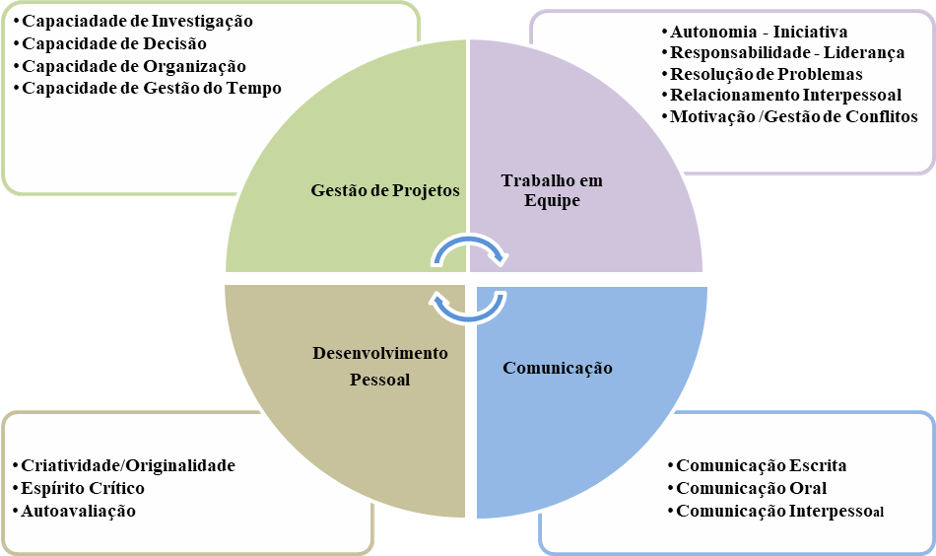
\includegraphics[width=\textwidth]{images/competencias_pbl.png}
  \end{figure}

Na PBL, a avaliação não se apresenta exclusivamente como um mecanismo de atribuição de nota, mas busca o feedback do aluno no que diz respeito às suas dificuldades no processo de aprendizagem (DELISLE, 2000; CARVALHO, 2009). Neste sentido, cada uma das etapas de desenvolvimento dos projetos será acompanhada de forma sistemática pelos professores.	
A próxima seção apresenta uma discussão mais ampla sobre a concepção de avaliação no âmbito deste projeto.

14.6. Avaliação do ensino e da aprendizagem

No decorrer da história da educação, foi atribuída à avaliação significados bastante diversos, resultantes das diferentes formas de conceber a relação entre ensino e aprendizagem. Apesar da pluralidade de definições e enfoques dados à avaliação, os estudos contemporâneos demonstram que avaliar para excluir ou meramente classificar a aprendizagem dos alunos está aquém do que de fato seriam as funções da avaliação (LUCKESI, 2003). Além disso, as práticas avaliativas exercidas pelos professores não podem ser entendidas em si mesmas, já que elas têm relação com as finalidades sociais mais amplas da educação.
	
Balizando-se por estas acepções, a avaliação no curso de Bacharelado em Ciência de Computação apresentará informações, em momentos diferenciados, acerca dos percursos de aprendizagens dos alunos e, também, sobre as práticas de ensino dos docentes (com vistas ao replanejamento do trabalho pedagógico). Esta compreensão é resultante do entendimento de que a avaliação atua como mediadora tanto do ensino quanto da aprendizagem (HOFFMAN, 2005). Assim, como uma atividade inerente à ação educativa, a avaliação:

\begin{enumerate}[label=(\alph*)]
    \item Estará	diretamente vinculada aos objetivos e às disciplinas do curso; 
    \item Ocorrerá de forma contínua, democrática, dinâmica, inclusiva, sistemática e intencional;
    \item Considerará as especificidades de cada componente curricular;
    \item Será pautada por critérios e instrumentos bem definidos;
    \item Servirá de informação para a melhoria não só do resultado, mas do processo de formação dos alunos.
    \item Levará	em conta as potencialidades dos estudantes considerando o real e não apenas o ideal.
\end{enumerate}

Evidentemente, cada tipo de conteúdo (conceitual, factual, procedimental e atitudinal) demanda formas específicas de ensinar e, por conseguinte, de avaliar. Conclui-se, portanto, a necessidade de os professores fazerem uso de variados instrumentos avaliativos apresentando, estes últimos, qualidade satisfatória, sob o risco de qualificar de forma inadequada os processos formativos dos discentes (SILVA, 2003). Portanto, os instrumentos escolhidos para atingir os objetivos pretendidos estarão adequados:

\begin{enumerate}[label=(\alph*)]
    \item Às competências e habilidades que estão sendo avaliadas;
    \item Aos conteúdos propostos e ministrados pelo docente; 
    \item À linguagem, de modo que o aluno possa compreender exatamente o que está sendo solicitado dele; 
    \item Ao processo de aprendizagem dos discentes.     
\end{enumerate}

No curso de Ciência da Computação, a avaliação ocorrerá, sistematicamente, durante todo o processo de ensino-aprendizagem, e não somente ao final de cada semestre. Por isso, será importante que não seja adotado, com exclusividade, uma única modalidade avaliativa (diagnóstica, processual ou somativa), mas que estas ocorram de forma articulada. Em determinados momentos poderão, ainda, ser estimuladas práticas de autoavaliação das aprendizagens, sendo estas condições didáticas importantes para a construção da autonomia dos estudantes.

QUADRO AQUI

O \textit{feedback} das avaliações constitui um aspecto fundamental no processo de acompanhamento do desenvolvimento do aluno, tendo em vista a construção, reconstrução e apropriação do conhecimento. Diante disso, também será assegurado aos estudantes o conhecimento dos pressupostos avaliativos que regem o curso de Bacharelado em Ciência de Computação, conforme o Parecer CNE/CES nº 236/2009.
	
A Universidade, por meio da Resolução CEPE/UFRPE nº494/2010, estabeleceu os procedimentos normativos no que tange ao registro das avaliações no âmbito do ensino da graduação. De acordo com este dispositivo, em cada disciplina serão realizadas três (3) verificações de aprendizagem e um exame final. Cada verificação de aprendizagem poderá ser feita através de uma única prova escrita ou de quaisquer outros instrumentos de avaliação, dependendo da natureza da disciplina e da orientação docente. As atividades avaliativas, além do seu caráter formativo e processual, terão, igualmente, um caráter cumulativo. Neste caso, “para efeito do cômputo do aproveitamento do aluno, nas verificações de aprendizagem e no exame final, serão atribuídas notas variando de zero (0) a dez (10), permitindo-se seu fracionamento em centésimos” (Art. 5º, §1º).

A frequência às aulas e demais atividades escolares será obrigatória, conside\-ran\-do-se reprovado na disciplina o aluno que não comparecer ao mínimo de 75\% (setenta e cinco por cento) das aulas ministradas (teóricas e práticas), ressalvados os casos previstos em lei (Art. 8º, Inciso I). Para fins de aprovação, além do mínimo de frequência exigido, o aluno deverá possuir média final igual ou superior a sete (7,0) em duas verificações da aprendizagem ou média final superior a cinco (5) entre a média de duas verificações de aprendizagem e a nota do exame final (Art. 7º, incisos I e II).

As disciplinas ministradas na modalidade EAD, terão suas avaliações na forma presencial, de acordo com a Portaria MEC nº 1.134/2016.

\section{Acessibilidade nos processos avaliativos}

Ainda no tocante à avaliação pedagógica, o curso de Bacharelado em Ciência da Computação encontra-se balizado, também, pela Política Nacional para Educação Especial na perspectiva da Educação Inclusiva (BRASIL, 2008). Nesta, a avaliação configura “uma ação pedagógica processual e formativa que analisa o desempenho do aluno em relação ao seu progresso individual, prevalecendo [\ldots] os aspectos qualitativos que indiquem as intervenções pedagógicas do professor”.

Com esse entendimento, o princípio da \textit{inclusão} norteará o processo de ensino e aprendizagem, garantindo que os professores, ao realizarem suas avaliações, promovam adaptações em função das necessidades educacionais especiais dos estudantes. Para os alunos que são considerados público-alvo da educação inclusiva (pessoas com deficiência, transtornos globais do desenvolvimento e com altas habilidades/superdotação), os docentes utilizarão, dentre outras estratégias, as seguintes adaptações avaliativas: \textit{dilatação de tempo de avaliação, apresentações de trabalhos em dupla, em equipes ou individual, prova oral, individualizada, sinalizada, ampliada, em Braile, em Libras, com recurso de tecnologias assistivas, permanência de profissional de apoio ou intérprete de Libras em sala e etc}.

É possível, assim, afirmar que, ao se adaptar uma avaliação ou uma estratégia didática, objetiva-se assegurar a equiparação de oportunidades, uma vez que todos os alunos são capazes de aprender, independente da sua idade cronológica, das suas limitações e de suas especificidades. Desse modo, o respeito à individualidade e ao tempo de cada um constitui um princípio fundamental para uma educação inclusiva.

\section{Integração entre as atividades de ensino, pesquisa e extensão}

Ensino, Pesquisa e Extensão constituem as áreas de atuação da Universidade e, conforme o disposto na Constituição Federal, em seu Art. 207, devem ser indissociáveis entre si. Neste sentido, o Programa de Educação Tutorial – PET, financiado pelo MEC, possibilita que os estudantes tenham uma ampla formação, na medida em que propõe o desenvolvimento de atividades que envolvem, de forma articulada, ensino, pesquisa e extensão. São alguns objetivos do Programa:

\begin{enumerate}[label=(\alph*)]
    \item Desenvolver atividades acadêmicas em padrões de qualidade de excelência, mediante grupos 	de aprendizagem tutorial de natureza coletiva e interdisciplinar;
    \item Contribuir para a elevação da qualidade da formação acadêmica dos alunos de graduação;
    \item Formular novas estratégias de	desenvolvimento e modernização do ensino superior no país;
    \item Introduzir novas práticas pedagógicas na graduação; 
    \item Contribuir com a política de diversidade na IES, por meio de ações afirmativas em defesa da equidade socioeconômica, étnico-racial e de gênero.
\end{enumerate}

	Na UFRPE existem 18 grupos PET organizados em quatro eixos (Original, Conexões Saberes, Engenharias e Interdisciplinar). No que tange à prática iniciação à pesquisa, esta é incentivada por meio do Programa Institucional de Bolsas de Iniciação Científica – PIBIC, financiado pelo Conselho Nacional de Desenvolvimento Científico e Tecnológico – CNPq, pela Fundação de Amparo à Ciência e Tecnologia do Estado de Pernambuco – FACEPE e pela própria Universidade. Dentre os objetivos do PIBIC, está o de:

\begin{enumerate}[label=(\alph*)]
    \item Despertar a vocação científica e incentivar novos talentos entre estudantes de graduação;
    \item Estimular uma maior articulação entre a graduação e pós-graduação;
    \item Estimular pesquisadores produtivos a envolverem alunos de graduação nas atividades científica, tecnológica e artístico-cultural;
    \item Proporcionar ao bolsista, orientado por pesquisador qualificado, a aprendizagem de técnicas e métodos de pesquisa, bem como estimular o desenvolvimento do pensar cientificamente e da criatividade, decorrentes das condições criadas pelo confronto direto com os  problemas de pesquisa;
    \item Ampliar o acesso e a integração do estudante à cultura científica.
\end{enumerate}

Outro importante exemplo é o Programa de Iniciação Científica – PIC, por meio do qual são concedidas cotas de orientação aos docentes/pesquisadores sem concessão de bolsas aos discentes. Trata-se de uma ação que amplia a formação de discentes/pesquisadores na instituição compartilhando dos objetivos do PIBIC. Já o Programa Institucional de Bolsas de Iniciação em Desenvolvimento Tecnológico e Inovação – PIBITI, financiado pelo CNPq, objetiva contribuir para a:

\begin{enumerate}[label=(\alph*)]
    \item Formação e inserção de estudantes em atividades de pesquisa,  desenvolvimento tecnológico e inovação;
    \item Formação do cidadão pleno, com condições de participar de forma criativa e empreendedora na sua comunidade;
    \item Formação de recursos humanos que se dedicarão ao fortalecimento da capacidade inovadora das 	empresas no Brasil.
\end{enumerate}

No curso de Ciência de Computação, a prática de iniciação à pesquisa também estará presente no cotidiano da “sala de aula”, na medida em que “aprender com pesquisa é um processo dialógico que envolve a problematização do conhecimento, a construção de argumentos e sua respectiva validação” (LAMPERT, 2008). Isso significa que o professor estimulará situações que possibilitem o questionamento sistemático de um determinado objeto, levando, em seguida, à elaboração de uma estrutura argumentativa com base na análise de diferentes fontes para, enfim, proceder às formas de divulgação dos resultados alcançados, tais como a redação de artigos e realização de seminários. Este processo envolve várias etapas e pressupõe um tempo e orientação específicos para a sua realização, de modo que o aluno possa desenvolver algumas aprendizagens fundamentais para a sua profissão, conforme destaca Masetto (2012, p. 118):

\begin{enumerate}[label=(\alph*)]
    \item Selecionar, organizar, comparar, analisar, correlacionar dados e informações;
    \item Fazer inferências, levantar hipóteses, checá-las, comprová-las, refutá-las e tirar conclusões;
    \item Elaborar um relatório.
\end{enumerate}

O ensino com pesquisa possibilita relacionar teoria e prática, além do desenvolver habilidades de comunicação e expressão oral e escrita. O tema da pesquisa pode estar articulado com vivências realizadas pelos estudantes e professores em projetos e programas desenvolvidos em parceria com ONGs, movimentos sociais, prefeituras, escolas, empresas, cooperativas, etc. Na UFRPE, o Programa Institucional de Bolsas de Extensão (BEXT) apoia projetos extensionistas nas temáticas de Saúde, Educação, Cultura, Tecnologia, Direitos Humanos, Trabalho, Meio Ambiente e Comunicação. Dentre os objetivos do BEXT, está o de:

\begin{enumerate}[label=(\alph*)]
    \item Estimular a participação de estudantes em ações de extensão, com vistas a promover a cidadania e a inclusão social, bem como a aprendizagem mediante a relação entre teoria e prática;
    \item Contribuir para a transformação social da comunidade-alvo;
    \item Priorizar a transferência de tecnologias capazes de proporcionar a sustentabilidade em comunidades localizadas, preferencialmente, na “zona rural” de Pernambuco. 	
\end{enumerate}

A extensão universitária constitui um elemento para “problematizar o ensino pela vivência presencial, solidária e transformadora” (PIVETTA et al, 2010). A articulação entre ensino e extensão pressupõe uma noção ampliada de “sala de aula”, incluindo “todos os espaços, dentro e fora da Universidade, em que se aprende e se (re)constrói o processo histórico-social em suas múltiplas determinações e facetas” (FORPROEX, 2012). Uma primeira consequência desse movimento é a geração de novas tecnologias e serviços oriundos da dialogicidade entre saberes acadêmicos e não acadêmicos. Outro efeito diz respeito ao impacto na formação dos futuros Bacharéis em Ciência da Computação a partir da percepção e do redimensionamento de conhecimentos, atitudes e valores em torno de sua profissão. Os professores deverão, portanto, estar atentos a esse contexto buscando locupletar o ensino por meio do engajamento com “problemas que são candentes à sociedade em que ela [a Universidade] está inserida” (SAVIANI, 1984).  
